Here's some TikZ code that creates a heart shape with the points and lines you described:
```
\documentclass[tikz,border=5mm]{standalone}
\begin{document}
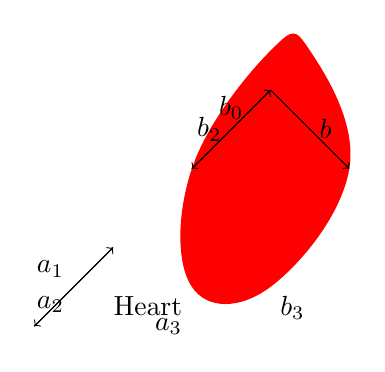
\begin{tikzpicture}
  % Draw the heart shape
  \fill[red] plot [smooth cycle, tension=0.7]
    coordinates {(0,0) (1,1.5) (1.5,1.5) (2,0) (1,-1.5) (0,-1.5)};
  
  % Draw the lines and points
  \draw[->] (0,0) -- node[midway,above] {$b_0$} (1,1);
  \draw[->] (1,1) -- node[midway,right] {$b$} (2,0);
  \draw[->] (1,1) -- node[midway,left] {$b_2$} (0,0);
  \node[below right] at (1,-1.5) {$b_3$};
  \draw[->] (-1,-1) -- node[midway,above left] {$a_1$} (-2,-2);
  \draw[->] (-2,-2) -- node[midway,below left] {$a_2$} (-1,-1);
  \node[left] at (0,-2) {$a_3$};
  
  % Add labels to the heart shape
  \node[below left] at (0,-1.5) {Heart};
\end{tikzpicture}
\end{document}
```
This code creates a heart shape using a smooth cycle path, and then draws lines and points as specified. You can adjust the positions and styles of the elements to fit your needs.